\chapter{Propuesta}

El fin de este trabajo es postular un modelo capaz de estimar los beneficios económicos asociados al uso del BIM en los proyectos de construcción industriales en CODELCO, en particular, generando una metodología que siente las bases para realizar estimaciones de los sobrecostos de los proyectos de construcción relativos al contexto de CODELCO respecto de su presupuesto inicial.

Sin embargo, esta propuesta también puede extenderse a otros contextos y tomarse como la base para generar estimaciones en cualquier tipo de industria que utilice la metodología BIM en sus proyectos de construcción.

\section{Métrica propuesta}

Las métricas propuestas por la literatura, en general, giran en torno al uso de contrafactuales, ya sea de comparando con otros proyectos similares que han utilizado la metodología BIM o bien haciendo una comparación con los beneficios teóricos que indica la literatura sobre el uso BIM.

En el primer grupo, por ejemplo, se tienen los siguientes estudios que son relevantes para el desarrollo de la propuesta de esta Memoria:

\begin{itemize}
    \item \citeA{barlish2012measure} proponen un método donde los indicadores propuestos permiten aventurar conclusiones en base a la comparación del nivel que estos alcanzaron en proyectos con BIM versus proyectos sin BIM. Sin embargo, una propuesta como esta tiene la desventaja de necesitar de un contrafactual para validarse.
    \item \shortciteA{lu2012generic} propone una métrica en la que el indicador es un parámetro derivado de otros indicadores, que son los esfuerzos (medidos en horas-hombre) y la superficie por unidad de trabajo (m$^2$ por piso, por ejemplo). Este método también cuenta con la desventaja de necesitar de un contrafactual para validarse.
\end{itemize}

Por otro lado, un ejemplo del segundo grupo es el siguiente estudio:

\begin{itemize}
    \item \citeA{saldias2010estimacion} proponen un método que permite levantar conclusiones en base a la cantidad de solicitudes de información (SDI) y órdenes de cambio que pudieron haberse evitado con el uso de la metología BIM. Este método tiene la desventaja de comparar proyectos sin BIM contra el ideal esperado con el uso de BIM (madurez óptima), sin tomar en cuenta los puntos intermedios de proyectos que utilizan al menos algún nivel de esta metodología.
\end{itemize}


Así, y en línea con lo planteado como fin de esta Memoria, es esencial que el método propuesto desestime el uso de un contrafactual para validarse, y busque, alternativamente, una manera de producir estimaciones de sobrecostos respecto de variables exógenas que se determinen dentro del modelo y en relación con otras variables internas.

La métrica a proponerse, entonces, debe:

\begin{enumerate}
    \item Desestimar el uso de un contrafactual y utilización de una variable exógena.
    \item Incluir cualquier nivel de adopción de la metodología BIM en el proyecto (madurez BIM).
\end{enumerate}

Así, en vez de construir un modelo en base a indicadores que pueden extraerse de manera directa de los reportes de los proyectos, el modelo propuesto utiliza una métrica que toma en cuenta el nivel de madurez BIM alcanzado (de acuerdo a una escala previamente determinada), el nivel óptimo de madurez y la desviación de los costos de los proyectos.

Asimismo, y dado que se espera que los costos de un proyecto crezcan en relación inversa al nivel de madurez BIM alcanzado por este, es necesario que el indicador se compare con respecto a su nivel de madurez óptimo. Formalmente, esto queda:

\begin{equation}
    \text{Indicador Madurez} = \frac{\text{Madurez BIM óptima}}{\text{Nivel de madurez BIM del proyecto}}
    \label{eq:indicador-propuesto}
\end{equation}

\section{Selección y generación de datos}

El proceso de generación de los datos finales sobres los cuales se realizará el análisis para generar la pripuesta se realiza a través de los procesos que muestran el siguiente diagrama:

\tikzstyle{startstop} = [rectangle, minimum width=3cm, minimum height=1cm, text centered, draw=black, fill=gray!5]

\begin{figure}[H]
    \centering
    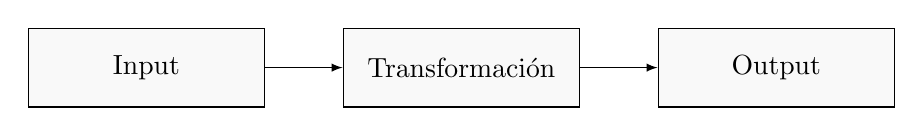
\begin{tikzpicture}[node distance=2cm]
        \node (in)  [startstop] {Input};
        \node (etl) [startstop, right of=in, xshift=2cm] {Transformación};
        \node (out) [startstop, right of=etl, xshift=2cm] {Output};

        \draw [-latex] (in) -- (etl);
        \draw [-latex] (etl) -- (out);
    \end{tikzpicture}
    \caption{Diagrama de generación de la data final.}
    \label{fig:data-final}
\end{figure}

\noindent
Donde,

\begin{table}[H]
    \begin{tabular}{l p{0.754\linewidth}}
        \textbf{Input:}          & es la data bruta (\emph{raw data}) sobre la cual se buscará y seleccionará la información relevante.\\
        \textbf{Transformación:} & la data ingresada pasa por un proceso de transformación que selecciona sólo la data de interés.\\
        \textbf{Output:}         & conjunto de datos finales sobre los cuales se realiza el análisis que sirve para proponer el método de estimación del crecimiento de los costos.
    \end{tabular}
\end{table}


\subsection{Criterio de selección de la fuente de la información}

La métrica propuesta \eqref{eq:indicador-propuesto} es la variable independiente del modelo que busca explicar el crecimiento de los costos de un proyecto de construcción en relación a su presupuesto inicial y de acuerdo al nivel de integración BIM (madurez BIM) que haya alcanzado un proyecto. 

Así, para generar un modelo es necesario conocer la información relativa a todos aquellos factores que devinieron en un aumento en los costos incialmente proyectados, y que bien pudieron evitarse de haberse utilizado e integrado el BIM de manera óptima.

De esta manera, la selección de los datos utilizados para relacionar estas variables y generar un modelo capaz de predecir la desviación en costos basasado en la métrica propuesta tiene dos fuentes principales desde las cuales era posible extraer la información interés: la primera es el reporte final de los proyectos con sus respectivos cambios y tendencias; la segunda es el Detalle de los Contratos de los proyectos.

Sin embargo, dado el nivel de detalle de la información contenida en cada una de las fuentes, se escogió el reporte con el Detalle de los Contratos como la base de extracción de datos.

\subsection{Input}

Se fija como \emph{input} la información contenida en el Detalle de los Contratos. Dicho reporte ofrece, adicionalmente, la ventaja de separar el detalle del costo base y el costo final. Esta clasficiación permite generar una estructuta de transformación de datos que ocurre de manera sistemática en orden detallado a continuación:

\begin{enumerate}
    \item \textbf{Crecimiento contratos:} en primer lugar, se selecciona una submuestra que contiene únicamente los contratos que experimentan un crecimiento en sus costos finales respecto del costo base del proyecto.
    
    \item \textbf{Crecimiento construcción:} luego, se considera sólo la información referida a los crecimientos de los costos de cada contrato en la fase de construcción.
    
    \item \textbf{Itemización BIM:} finalmente, se separa la información por ítems relacionados al uso (o falta de uso) de la metodología BIM. La itemización BIM se compone de los siguientes ítems: extensión de plazo, obras adicionales, materiales e ingeniería.
\end{enumerate}

La selección de información asociada a cada uno de los ítems de la itemización BIM puede variar según el proyecto. Sin embargo, para el caso de los proyectos analizados en este estudio, las palabras clave para dicha selección eran coincidentes entre proyectos. Esto dado que quienes crean el reporte son parte de la misma Dirección (Dirección de Contratos de la Vicepresidencia de Proyectos) y de la misma compañía (CODELCO).

Se tiene, entonces, que para el filtrado por ítem, las palabras clave fueron:

\begin{table}[H]
    \centering
    \caption{Palabras clave para la selección de cada ítem asociado al BIM.}
    \label{tab.keyw}
    \begin{tabular}{ll}
        \toprule
        \textbf{Ítems}      & \textbf{Palabras clave} \\
        \midrule
        Extensión de plazo  & Extensión plazo, plazo\\
        Obras adicionales   & Montaje, obras adicionales, rellenos, reemplazos, reparaciones, etc.\\
        Materiales          & Hormigón, piping, cañerías, cables, válvulas, etc. \\
        Ingeniería          & Ingeniería, ingeniería de terreno, etc. \\
        \bottomrule
    \end{tabular}
\end{table}

\subsection{Transformación}

La transformación ocurre a través de una pieza de \emph{software} desarrollada en Python que obedece a la lógica que se detalla a continuación:

Primero, los datos ingresados son seleccionados de acuerdo a la condición,

\begin{equation}
    C_{fi} > C_{0i}
\end{equation}

\noindent
Donde,\\
$C_{fi}$: costo final del proyecto $i$.\\
$C_{0i}$: costo inicial del proyecto $i$.

Para efectos de esclarecimiento, se denomirá este set de datos como $DC_i$. A continuación, desde $DC_i$ se extraen solamente los datos de los contratos asociados a la contrucción del proyecto $i$. Ests subconjunto será denomida como $CC_i$ y cumple con la condición:

\begin{equation}
    CC_i \subset DC_i
\end{equation}

Finalemte, desde $CC_i$ se extrean los datos para cada ítem de la itemización BIM, tal que:

\begin{equation}
    \text{itemización BIM} \in CC_i
\end{equation}

\subsection{Output}

El \emph{output} del proceso de transformación de la data da como resultado el siguiente desglose en términos porcentuales para cada uno de los proyectos estudiados. Así, las desviaciones en costos para los proyectos estudiados en este trabajo se distribuyen de acuerdo a lo mostrado en la siguiente Tabla:

\begin{table}[H]
    \centering
    \label{tab.datos_desv_proy}
    \caption{Desviaciones en costo de los proyectos estudiados.}
    \begin{tabular}{lccc}
        \toprule 
        Ítem              & Ministro Hales   & Moly corporativo & Planta de Ácido \\
        \midrule
        Extensión plazo   & 2,0 \%           & 5,4 \%           & -       \\
        Obras adicionales & 19,7 \%          & 2,4 \%           & 5,6 \%  \\
        Materiales        & 3,2 \%           & 8,1 \%           & 5,9\%   \\       
        Ingeniería        & 0,08 \%          & 0,12 \%          & 0,3 \%  \\
        \hline
        \textbf{Total}    & \textbf{24,9} \% & \textbf{16,2} \% & \textbf{11,8} \% \\
        \bottomrule
    \end{tabular}
\end{table}

\subsection{Herramienta de selección y generación de base de datos}

El reporte con el Detalle de los Contratos es una planilla Excel con varios miles de datos, por lo que el filtrado a través de Excel es poco conveniente y susceptible a errores. Por esta razón, se desarrolló un código en Python capaz de seleccionar y transformar los datos requeridos a través de una pseudo minería de datos. Dicho código está disponible en el siguiente repositorio GitHub \url{www.github.com/psotou/contract-data-selection.git}

Cabe mencionar que si bien el código se creó para trabajar con cualquier reporte de Detalle de Contratos emitidos por la Vicepresidencia de Proyectos de CODELCO, basta con ajustar algunos parámetros para que dicho código pueda usarse con un reporte de similares características de cualquier otra empresa o institución.


\subsection{Evaluación de madurez BIM de los proyectos}

La evaluación del nivel de madurez BIM alcanzado por cada uno de los proyectos estudiados realizada por Marcelo Vásquez, quien fue la persona encargada de la coordinación BIM de todos estos proyectos en CODELCO.

Marcelo utilizó la metodología desarrollada por \citeA{succar2010building} y utilizó la matriz de madurez que el autor propone para entregar el \emph{rating} asociado a cada proyecto según los niveles establecidos en la Tabla \ref{tab:niveles-madurez-codelco}. Bajo este contexto, la evaluación de Marcelo Vásquez para los proyectos fue la siguiente:

\begin{table}[H]
    \centering
    \caption{Nivel de madurez BIM de cada proyecto según \emph{rating} evaluado por especialista.}
    \label{tab:evaluacionmadurez}
    \begin{tabular}{lc}
        \toprule 
        \textbf{Proyecto} & \textbf{Nivel de madurez BIM} \\
        \midrule
        Ministro Hales   & 1,7 \\
        Moly corporativo & 1,8 \\
        Planta de ácido  & 2,2 \\
        \bottomrule
    \end{tabular}
\end{table}

\section{Aplicación de la métrica propuesta}

Al tranformar los datos de la Tabla \ref{tab:evaluacionmadurez} de acuerdo a la métrica propuesta \eqref{eq:indicador-propuesto}, el conjunto de datos sobre los que se levanta la propuesta de este estudio queda como se muestra a continuación:

\begin{table}[H]
    \centering
    \caption{Base final que muestra el crecimiento de los costos junto a su respectivo indicador madurez (métrica propuesta).}
    \label{tab:datosfinales}
    \begin{tabular}{lccc}
        \toprule 
        \textbf{Proyecto}  & \textbf{Desviación} & \textbf{Nivel de madurez} & \textbf{Indicador madurez} \\
        \midrule
        Ministro Hales     & 24,9 \%             & 1,7                       & 2,35 \\
        Moly corporativo   & 16,2 \%             & 1,8                       & 1,82 \\
        Planta de ácido    & 11,8 \%             & 2,2                       & 2,22 \\
        \bottomrule
    \end{tabular}
\end{table}


En base a la información de la Tabla \ref{tab:datosfinales} se construye la propuesta de un modelo que permite realizar estimaciones del crecimiento de los costos de un proyecto de acuerdo a su nivel de madurez BIM alcanzado.

%-----------------------------MODELO TEÓRICO----------------------
\section{Teoría detrás del modelo propuesto}

En términos generales, la relación entre el crecimiento de los costos de un proyecto $i$ y los factores que lo motivan se puede expresar de la siguiente manera:

\begin{equation}
    \label{eq.desv-gen}
    y_i = \theta_0 +\sum\limits_{i=1}^n \theta_i x_i
\end{equation}

O bien, de manera vectorial:

\begin{equation}
    \label{eq.desv-vec}
    y_i = \bm{x}^T_i\bm{\theta}
\end{equation}

Donde tanto $y_i$ como $\bm{x}_i$ son variables observadas. Se asumirá que $\varepsilon_i$ (término de error o de perturbación no observado) es absorbido por la constante $\theta_0$. Aquí, $\bm{x}^T$ es un vector fila cuyos elementos son los indicadores de madurez propuestos $(1,~x_1,~x_2,\ldots,~x_n)$, y $\bm{\theta}$ es un vector columna con $(\theta_0,~\theta_1,~\theta_2,\ldots,~\theta_n)^T$  paramámetros desconocidos que son los que se desea estimar con el fin de poder generar un modelo que sirva como base para explicar la influencia de factores tales como el uso de alguna nueva metodología (que es el caso de este estudio), en el crecimiento de los costos de un proyecto.

Para efectos de esta Memoria, $y_i$ representa los crecimientos de los costos de cosntrucción para el proyecto $i$, y $\bm{x}_i$ representa la métrica propuesta como indicador de madurez en la \eqref{eq:indicador-propuesto}.


Adicionalmente, la ecuación \eqref{eq.desv-vec} se puede escribir usando notación matricial:

\begin{equation}
    \label{eq.matrix}
    \bm{y} = X\bm{\theta} + \varepsilon
\end{equation}

Donde $\bm{y}$ y $\varepsilon$ son vectores de dimensiones $(N\times1)$, $X$ es una matriz de dimensión $(N\times K)$ y $\bm{\theta}$ un vector de dimensión $(K\times1)$. Esta será la forma que se utlizará para hace el ingreso de la data a la pieza de \emph{software} desarrollada. Aquí también se considera el supuesto en que el vecto de errores $\varepsilon$ es absorbido por el vector $\bm{\theta}$, de manera que la ecuación sobre la que se trabajará queda de la siguiente manera:

\begin{equation}
    \label{eq:matricial-final}
    \bm{y} = X\bm{\theta}
\end{equation}

Antes de comenzar con la estimación de los parámetros de interés $\bm{\theta}$, se deben levantar algunos supuestos para darle significado al modelo de manera que este no carezca de sentido estadístico. En primer lugar, se asume que las variables explicativas $\bm{x}_i$ son exógenas, lo que implica que $\bm{E}[y_i|\bm{x}_i]=0$. Bajo este supuesto, se sostiene que :

\begin{equation}
    \label{eq.e-xb}
    \bm{E}[y_i|\bm{x}_i] = \bm{x}_i^T\bm{\theta}
\end{equation}

De manera que la curva $\bm{x}_i^T\bm{\theta}$ describe la esperanza condicional de $y_i$ dados los valores de $\bm{x}_i$, y los coeficientes de $\bm{\theta}$ miden cuánto cambia el valor esperado de $y_i$ si cambia un valor $x_{ik}$ (siendo éste el $k$-ésimo elemento del vector $\bm{x}_i$) manteniendo todos los otros elementos de $\bm{x}_i$ constantes (condición ceteris paribus) \cite{verbeek}.

Los parámetros de $\bm{\theta}$ se estimarán on el estimador de Mínimos Cuadrados Ordinarios (MCO). Utilizando la notación de la ecuación \eqref{eq.matrix}, el estimador está dado por:

\begin{equation}
    \label{eq.mco}
    \bm{\hat\theta} = \left( X^TX\right)^{-1}X^T\bm{y}
\end{equation}

Luego, la predicción de valores de desviación vendrá dada por:

\begin{equation}
    \label{eq.predicc}
    \hat{\bm{y}} = X\hat{\bm{\theta}}
\end{equation}

Donde $\hat{\bm{y}}$ son las predicciones de las desviaciones dada la estimación de los parámetros de $\bm{\theta}$.  

La muestra sobre la cual se funda este estudio consiste de un conjunto muy reducido de datos, por lo que se utilizará MCO para muestra pequeña. Las propiedades del estimador MCO para muestra pequeña son:

\begin{align}
    & \label{eq.s1} \bm{E}[\varepsilon_i] = 0\\
    & \label{eq.s2} \varepsilon_i\quad\text{independiente de}\quad \bm{x}_i\\
    & \label{eq.s3} \bm{V}[\varepsilon_i]=\sigma^2 \\
    & \label{eq.s4} \text{cov}[\varepsilon_i,~\varepsilon_j] = 0,\quad i\neq j
\end{align}

El supuesto \eqref{eq.s1} indica que el valor esperado del término de error es cero, esto significa que, en promedio, la curva de regresión debería estar correcta. 

El supuesto \eqref{eq.s3} indica que todos los términos de error poseen la misma varianza, esto se conoce como homoceasticidad.

El supuesto \eqref{eq.s4} impone cero correlación entre los términos de error, excluyende así cualquier forma de autocorrelación. Usando la notación matricial, estos tres supuesto se pueden reescribir de la siguiente forma:

\begin{equation}
    \bm{E}[\varepsilon]=0\quad\text{y}\quad\bm{V}[\varepsilon]=\sigma^2I_N
\end{equation}

Con $I_N$ matriz identidad de dimensiones $(N\times N)$. Esto muestra que la matriz de covarianza del vector de los términos de error $\varepsilon$ es una matriz diagonal con $\sigma^2$ en la diagonal.

El supuesto \eqref{eq.s2} indica que $X$ e $\varepsilon$ son independientes. Este es un supuesto fuerte que implica:

\begin{equation}
    \bm{E}[\varepsilon|X]=\bm{E}[\varepsilon]=0
\end{equation}
\begin{equation}
    \bm{V}[\varepsilon|X]=\bm{V}[\varepsilon]=\sigma^2I_N
\end{equation}

Es decir, la matriz de regresores $X$ no provee ninguna información sobre los valores esperados de los términos de error o sus (co)varianzas. 

Una propiedad muy relevante del estimador de mínimos cuadrados es que se trata de un \textbf{estimador insesgado}. Esto quiere decir que, en promedio, se espera que los valores del estimador $\bm{\hat\theta}$ sean iguales a los valores verdaderos de $\bm{\theta}$ \cite{verbeek}. Formalmente, esto es:


\begin{equation}
    \bm{E}[\hat{\bm{\theta}}] = \bm{\theta}
\end{equation}

Hasta ahora se ha descrito la interpretación del modelo para un valor esperado de $y_i$ dados los valores observado de las variables explicativas $\bm{x}_i$.

Además de ese análisis, es importante conocer el \textbf{efecto marginal} de dichas variables sobre el valor esperado de $y_i$. En otras palabras, en cuántas unidades se espera que cambie $y_i$ si $x_{ik}$ cambia en una unidad siempre que el resto de las variables en $\bm{x}_i$ se mantenga constante (condición ceteris paribus) \cite{hansen2018}. Esta medida viene dada por:

\begin{equation}
    \label{eq.efec_marginal}
    \frac{\partial \bm{E}[y_i|\bm{x}_i]}{\partial x_{ik}} =\theta_k
\end{equation}

%--------------------------MODELO EMPÍRICO---------------
\section{Modelo propuesto}

La coordinación digital de un proyecto de construcción a través del uso de la metodología BIM supone reducir los costos asociados a errores, interferencias, omisiones, etc, por lo que a medida que el grado de integración de la metodología en el proyecto crece, los costos asociados a los problemas mencionados disminuyen.

Dado este escenario, es de esperarse que el uso del BIM impacte de manera postiva en el ahorro en costos de construcción de un proyecto. Se desprende, entonces, que un proyecto que alcanza un buen nivel de madurez BIM debería tener un sobre costo menor al esperado en un proyecto realizado sin BIM.

Por lo anterior, la hipótesis sobre la que se basa esta propuesta es que la desviación de los costos de un proyecto es inversamente proporcional a su grado de madurez BIM. Para ello, se define la variable explicativa $x_{ik}$ de la siguiente manera:

\begin{equation}
    x_{ik} = \frac{m}{m_i}
\end{equation}

Donde $m$ es el óptimo de madurez BIM, y $m_i$ es el nivel de madurez BIM alcanzado por el proyecto $i$. Aquí, $x_{ik}$ no es otra cosa que la métrica propuesta en \eqref{eq:indicador-propuesto}.

Con esto, la ecuación \eqref{eq.desv-gen} queda:

\begin{equation}
    \label{eq:modelo-propuesto}
    y_i = \theta_0 + \sum\limits_{i=1}^n \theta_i \left(\frac{m}{m_i} \right)
\end{equation}

Además, la desviación en los costos de un proyecto está sujeta las siguientes condiciones de borde de acuerdo a la NBS-UK \cite{nbs}:

\begin{equation}
    y_i = 
    \begin{cases}
        0,33 & \text{si}~~ m_i = m_{\text{máx}} \\
        0,001 & \text{si}~~ m_i = m_{\text{mín}}
    \end{cases}
\end{equation}

Esto valores son referenciales dado que consideran una integración óptima (máxima madurez BIM posible) de la metodología BIM.


\subsection{Estimación del modelo según la muestra}

La muestra de la que se disponía y sobre la que se trabajó consistía de tres proyectos minero-industriales, dos de estos proyectos de construcción \emph{greenfield} mientras que el otro, un proyecto \emph{brownfield} (Planta de ácido) de \emph{overhauling}.

Ahora, ingresando los datos de los crecimientos de los costos y el indicador de madurez estimado según \eqref{eq:indicador-propuesto} de toda la muestra, se generan las siguientes matrices:

\begin{minipage}{.45\linewidth}
    \begin{equation*}
    Y = 
        \begin{bmatrix}
            0,330 \\
            0,249 \\
            0,161 \\
            0,118 \\
            0,001 
        \end{bmatrix}
    \end{equation*}
\end{minipage}
\begin{minipage}{.45\linewidth}
    \begin{equation*}
    X = 
        \begin{bmatrix}
            1 & & 4,000 \\
            1 & & 2,353 \\
            1 & & 1,818 \\
            1 & & 2,222 \\
            1 & & 1,000
        \end{bmatrix}
    \end{equation*}
\end{minipage}

Lo que produce el siguiente estimador:

\begin{equation}
    \hat{\bm{\theta}} = 
        \begin{bmatrix}
            -0,0746 \\
            ~~~0,1083
        \end{bmatrix}
\end{equation}

Con lo que la relación entre desviación y madurez se modela como sigue:

\begin{equation}
    \label{eq.modelo-prop-todos}
    \hat{y_i} = -0,0746 + 0,1083\cdot \left( \frac{4}{m_i} \right)
\end{equation}

Cuyo efecto marginal sobre la desviación esperada de los costos es $0,1083$ según se estima a través de la ecuación \eqref{eq.efec_marginal}. Es decir, por cada una unidad de madurez BIM se espera una reducción en la desviación esperada de aproximadamente un $10,83\%$.

El gráfico asociado a la ecuación \eqref{eq.modelo-prop-todos} es:

\begin{figure}[H]
    \centering
    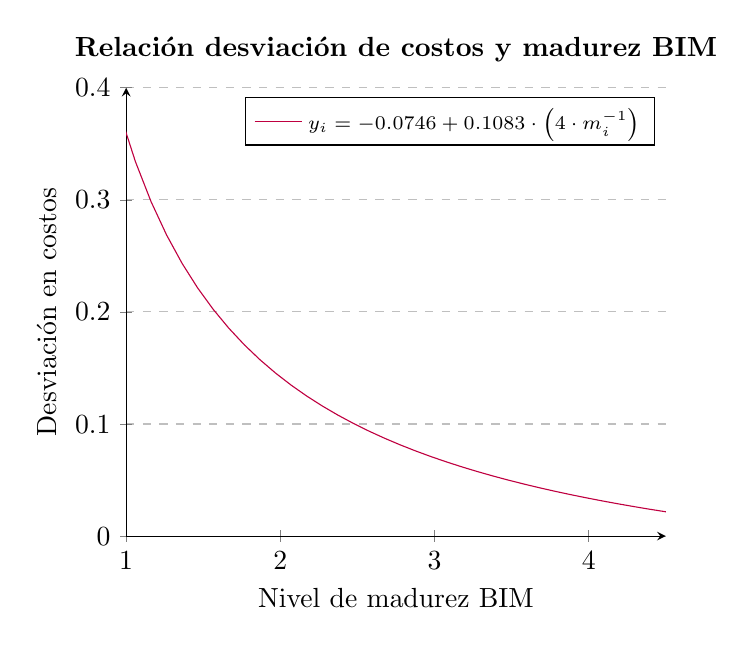
\begin{tikzpicture}
        \begin{axis}[
            axis lines = left,
            title = {\textbf{Relación desviación de costos y madurez BIM}},
            ymin = 0, ymax = 0.4,
            xmin = 1, xmax = 4.5,
            xtick = {1, 2, 3, 4},
            ymajorgrids = true,
            grid style = dashed,
            ylabel = Desviación en costos,
            xlabel = Nivel de madurez BIM,
            legend style = {font=\scriptsize},
         ]
        \addplot [
            samples = 100,
            color = purple,
         ]
         {-0.0746 + 0.1083 * 4 / x};
         \addlegendentry{$y_i = -0.0746 + 0.1083\cdot \left( 4 \cdot m_i^{-1} \right)$}
        \end{axis}
    \end{tikzpicture}
    \caption{Predicción de la desviación en costos en base a la muestra total.}
\end{figure}

Y las estadísticas asociadas al coeficiente que acompaña al indicador de madurez BIM (las cuales se generan a través de la pieza de \emph{software} desarrollada) se muestran en la siguiente Tabla:

\begin{table}[H]
    \centering
    \label{tab.est}
    \caption{Estadísticas asociadas al coeficiente de madurez BIM $\theta_1$.}
    \begin{tabular}{lccc}
        \toprule
        Coeficiente & error estándar & $p$-value & $R^2$\\
        \midrule
        0,1083      & 0,022          & 0,015     & 0,893\\  
        \bottomrule        
    \end{tabular}
\end{table}

%------------RESULTS ANALYSIS----------------
\subsection{Análisis de Resultados}

La propuesta de este estudio es proponer una metodología que permita generar un modelo capaz de estimar los crecimientos de los costos de construcción de un proyecto de acuerdo al nivel de madurez BIM alcanzado por dicho proyecto. 

Además, se sostiene la hipótesis de que, efectivamente, existe una relación inversa entre el nivel de madurez BIM de un proyecto y los crecimientos de los costos de construcción. Formalmente:

\begin{table}[H]
    \begin{tabular}{l p{0.9\linewidth}}
        $H_0$: & La madurez BIM no tiene un efecto inversamente proporcional en el crecimiento de los costos de construcción de un proyecto. \\

        $H_1$: & La madurez BIM sí tiene un efecto inversamente proporcional en el crecimiento de los costos de construcción de un proyecto.
    \end{tabular}
\end{table}

Donde $H_0$ es la hipótesis nula y $H_1$ la hipótesis alternativa. 

Para validar el modelo propuesto en términos estadísticos se debe contar con evidencia suficiente para rechazar $H_0$. La manera de corroborar dicha información es tomando en cuenta el valor que muestra el $p$-value. Puesto de otra manera, si $p<0,05$ existe evidencia para rechazar $H_0$; de lo contrario, si $p>0,05$, la evidencia en contra de $H_0$ es débil y no se puede rechazar. 

En este caso, y a pesar de lo limitada de la muestra, se tiene que $p<0,05$, por lo que se puede decir que existe evidencia para rechazar $H_0$ en favor de $H_1$, indicando así que existe evidencia estadística para validar la hipótesis de la relación inversa entre madurez BIM y el crecimiento de los costos.

Así, tomando en cuenta el resultado arrojado por la muestra total, el modelo representado en la ecuación \eqref{eq.modelo-prop-todos} demuestra que tanto la metodología como el indicador de madurez propuesto es una buena manera de estimar el crecimiento de los costos de contrucción de un proyecto. 

Sin embargo, y a pesar de que si bien el resultado de la muestra total se condice con lo esperado en teoría, ha de tenerse en cuenta que se utilizó una muestra bastante acotada, por lo que se debe tener el cuidado pertinente si se quiere generalizar sobre este resultado. No obstante, el modelo propuesto se comporta de manera bastante apropiada y viene a validar, en términos cuantitavos, aquella \emph{sensación} de ahorro que genera la utilización de la metodología BIM.